\chapter{Retrospective analyzer system}

This chapter is focused on the complementary software that has been added to this master thesis. Building on the approaches introduced in the chapter \nameref{ch:retroDedGams} and the ones actually implemented in Intel Technology Poland site presented in the chapter \nameref{ch:gamesDepl}, we created a web service, which helps scrum masters to chose a game suitable for the team.
The Retrospective analyzer system was created especially for Scrum Masters, Team Leaders and Managers in order to help them find suitable game for the retrospective meeting. Leading a team is a difficult assignment, but thanks to Scrum this job is being simplified. In order to ease it even more, we created the system that chooses a retrospective game for the team. What is more, we created a base of verified games with descriptions, in order to present a user what retrospective techniques our system provides. 

\section{System overview}

The Retrospective analyzer application is a web service, on the \autoref{fig:welcomePage} the welcome page is presented with the introduction what the system is offering.

\begin{figure}[h]
\caption{Welcome page screenshot}
\label{fig:welcomePage}
\centering
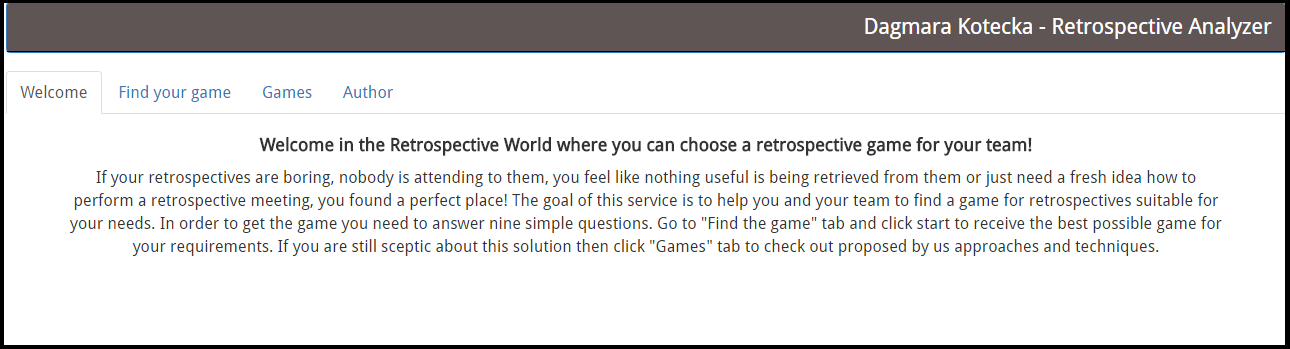
\includegraphics[width=1\textwidth]{screenshots/welcome.png}
\end{figure}

The Games tab is presented on the \autoref{fig:gamesPage} and it contains all the games included in this system.

\begin{figure}[h]
\caption{Games page screenshot}
\label{fig:gamesPage}
\centering
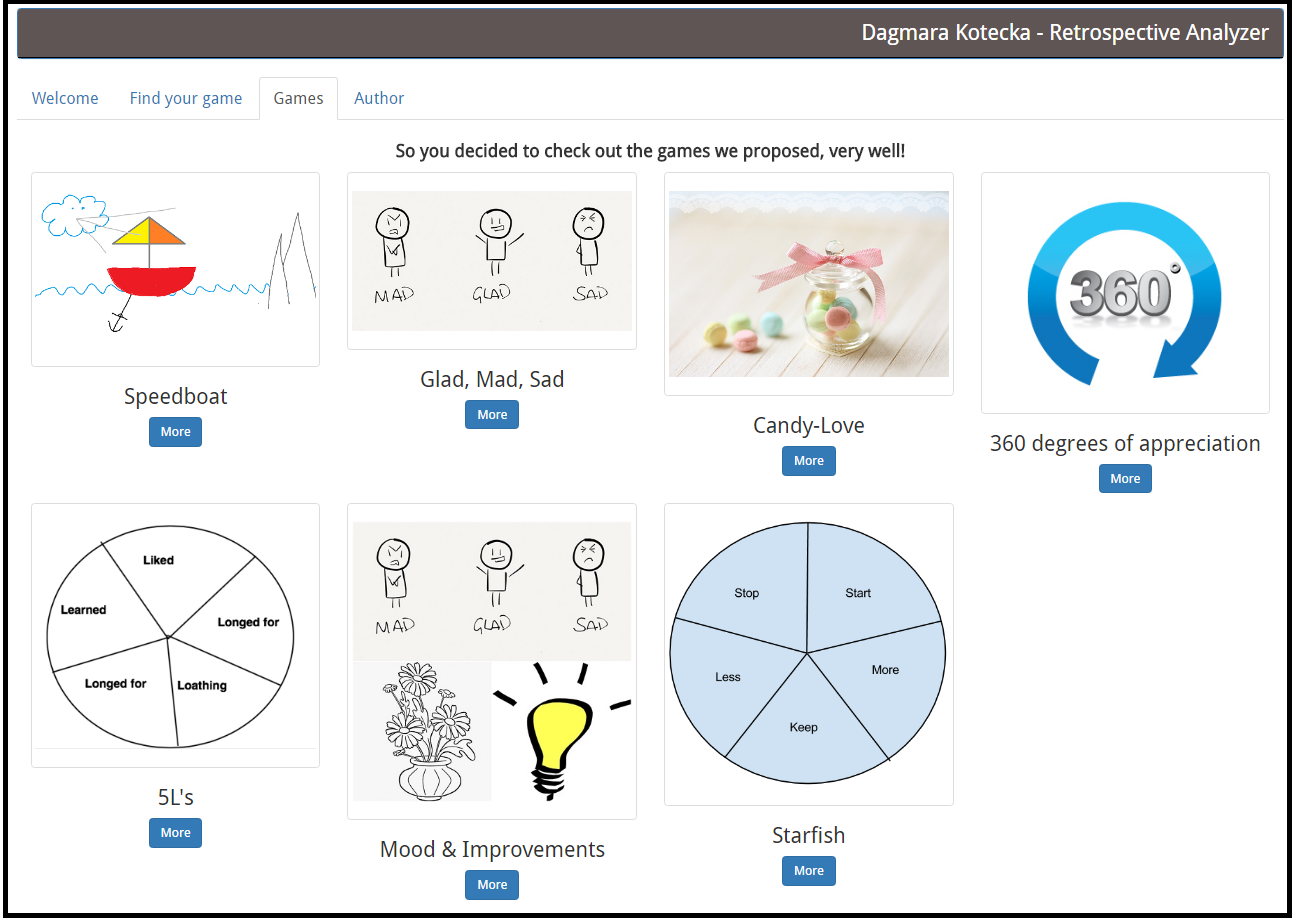
\includegraphics[width=1\textwidth]{screenshots/games.png}
\end{figure}

Another subpage and most important one is the Find The Game tab, where the main functionality of the system is introduced and from this place after clicking start button shown on the \autoref{fig:findGame} the user is being redirected to the page with questions presented on the \autoref{fig:questionsPage}. The question page corresponds to the main issues which may occur in the Scrum team, basing on users answers the system chooses the suitable retrospective approach.

\begin{figure}[h]
\caption{Find game screenshot}
\label{fig:findGame}
\centering
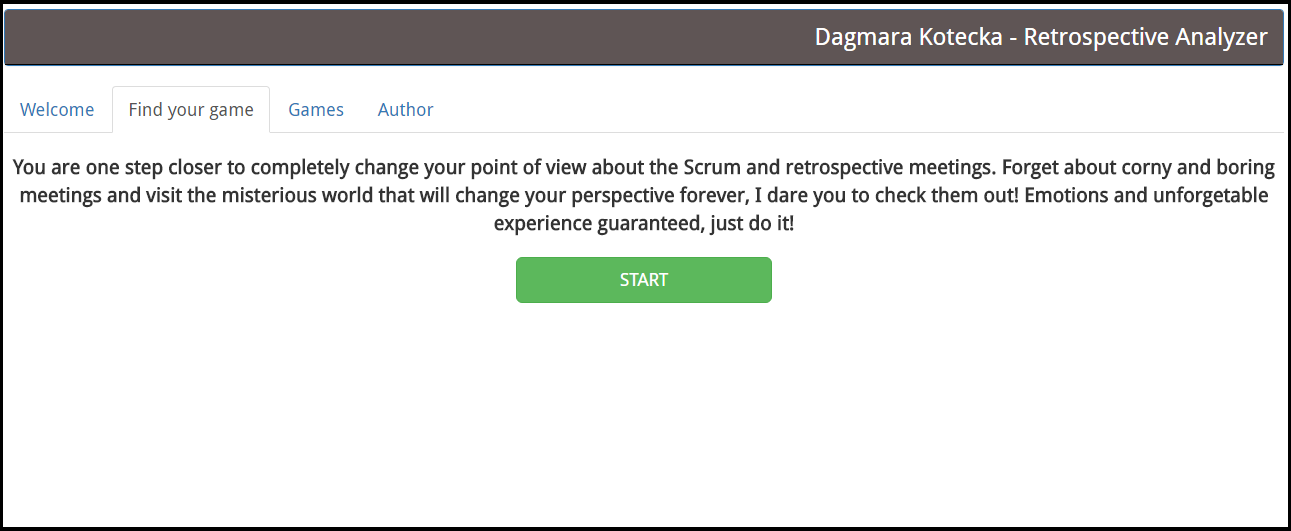
\includegraphics[width=1\textwidth]{screenshots/find.png}
\end{figure}

\begin{figure}[h]
\caption{Questions page screenshot}
\label{fig:questionsPage}
\centering
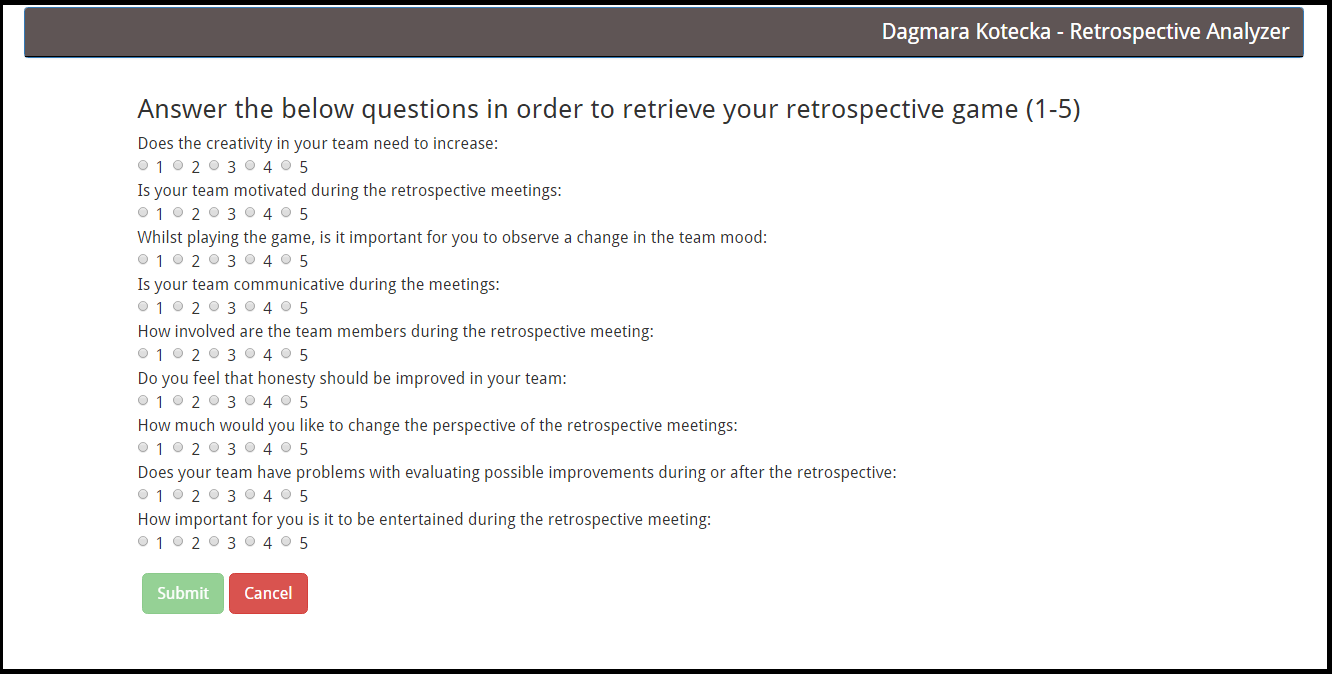
\includegraphics[width=1\textwidth]{screenshots/questions.png}
\end{figure}

The questions in the set were created based on the \autoref{fig:gamesPoints}, which presents how many points in scale from 1 to 10, where 1 is the lowest and 10 the highest value, the game reached in the particular factor. The table has been created in association with Grzegorz Reglinski, the Intel Technology Scrum Master, and we evaluated it basing on the feedback from the teams, on our scrum experience and on the data collected from the survey.

Overall the highest sum was granted to the 360-degrees of appreciation, the lowest amount of point received Glad, Mad, Sad. The rest of games' summary points fluctuates around value 50.

The chosen factors included in the table presented on the \autoref{fig:gamesPoints} are as follows:
\begin{enumerate}
    \item Creativity - how the game influences the creativity of the team members.
    \item Team mood - this factor is useful for the team leaders and managers, thanks to it, they are able to notice what is the team mood and react.
    \item Collaboration - this characteristic applies to how the game affects the cooperation of team members while performing retrospective meeting. 
    \item Communication - this element indicates whether the proposed approach enhances the discussions during the meeting.
    \item Involving - shows whether the proposed game increases the involvement of the participants.
    \item Change of perspective - indicates how different is the approach comparing to the standard procedures and how big is the impact of the proposed in the game change of perspective.
    \item Honesty - this indicates whether while using the game we can observe the increase of the honesty along the participants.
    \item Entertainment - this factor presents how much amusement the game brought to the retrospective meeting.
    \item Improvement - indicates how much the game supports the team in case of retrieving ideas for improvements.
\end{enumerate}

Moreover, the nine factors above indicates what game will be retrieved after answering using scale 1-5, where 1 is user definitely does not agree and 5 is definitely agree, the nine questions below (also presented on \autoref{fig:questionsPage}):
\begin{enumerate}
    \item Does your team need creativity increase?
    \item Is your team motivated during the retrospective meetings?
    \item Is it important for you to retrieve team mood, while playing?
    \item Is your team communicative in the meetings?
    \item How involved in the retrospective meeting are the team members?
    \item Do you think that honesty should be improved in your team?
    \item How much would you like to change the perspective of the retrospective meetings?
    \item Does your team has problems with evaluating the improvements during/after retrospective?
    \item How important for you it is to be entertained during the retrospective meeting?
\end{enumerate}

The implemented algorithm of choosing the game is written in JavaScript and is presented below in \autoref{lst:jsAlg}:

\begin{lstlisting}[float=ht,escapechar=@,
    language=JavaScript,
    caption={The algorithm of choosing the game in JavaScript},
    label={lst:jsAlg},
    basicstyle=\ttfamily,
    keywordstyle=\color{blue}\ttfamily,
    stringstyle=\color{red}\ttfamily,
    captionpos=b,
    aboveskip=20pt,
    frame=trbl]

while (arr.indexOf("1") !== -1 || arr.indexOf("2") !== -1 ||
        arr.indexOf("3") !== -1 || arr.indexOf("4") !== -1 || 
        arr.indexOf("5") !== -1) {
        getMaxIndexes(arr, function () {
            changeMaxToZero(function () {
                getGames(function () {
                    reduceGames();
                });
            });
        })
    }
    
\end{lstlisting}

The server receives the data and parses it into the temporary array \textit{arr}. Afterwards it is passed into the while loop with the condition - execute until the array will not contain 1-5 values. First function \textit{getMaxIndexes} retrieves from the array indexes of the elements that have the maximum value and in the \textit{changeMaxToZero} procedure sets the proper array element to 0. After taking those indexes, there are being mapped to the factors defined in \autoref{fig:gamesPoints} in the \textit{getGames} function and the ones with the 
\[factorsValue >= (MAX * 2) - 1\]
are being saved and stored in a global \textit{tmpArray} array along with the \textit{max} value. If the \textit{returnGames} array is empty then the \textit{reduceGames} function assigns the \textit{tmpArray} to the \textit{returnGames}. When the \textit{returnGames} array is not empty, it sums the \textit{max} with the already stored in it value
\[value[i] = value[i] + max  \].

If the array does not contain 1-5 values the game with the highest weight is being retrieved and:
\begin{enumerate}
    \item If the \textit{returnGames} array has more than 1 element, then the all of the games are viewed to the user.
    \item If the \textit{returnGames} array contains 1 element, the game is shown to the user.
\end{enumerate}

The source of this system has been open-sourced and can be found under this link \url{https://github.com/dagkotecka/Retrospective-Analyzer}.

\begin{figure}[h]
\caption{Games points table}
\label{fig:gamesPoints}
\centering
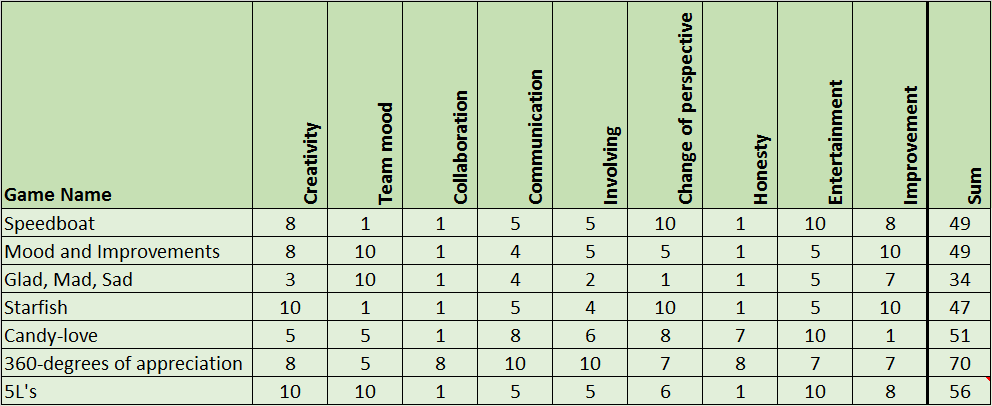
\includegraphics[width=1\textwidth]{screenshots/gamesPoints.png}
\end{figure}

After the user answers the questions, the system returns the game and a reference (as a button) to its description. This page is presented on the \autoref{fig:retrievedGame}.

\begin{figure}[h]
\caption{Retrieved Game page screenshot}
\label{fig:retrievedGame}
\centering
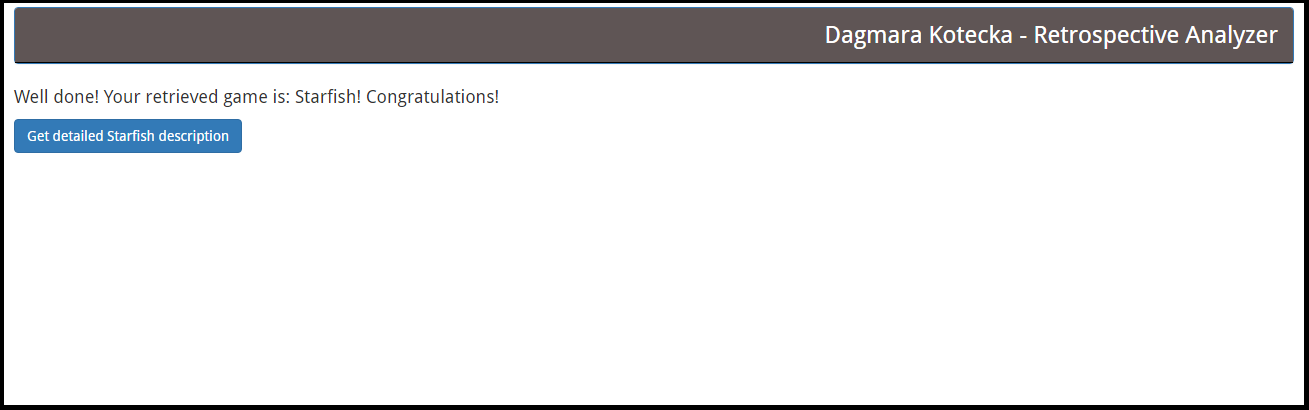
\includegraphics[width=1\textwidth]{screenshots/retrievedGame.png}
\end{figure}

There are two ways of entering the game description page shown on the \autoref{fig:gameDescPage}, first way is to access it via Games Page (\autoref{fig:gamesPage}), another option is, after filling the form on the questions page and retrieving the game from the system, by clicking the description button on the Retrieve Game page (\autoref{fig:retrievedGame}). The game description contains game name, rules and expected goal after performing. 

\begin{figure}[h]
\caption{Game description page screenshot}
\label{fig:gameDescPage}
\centering
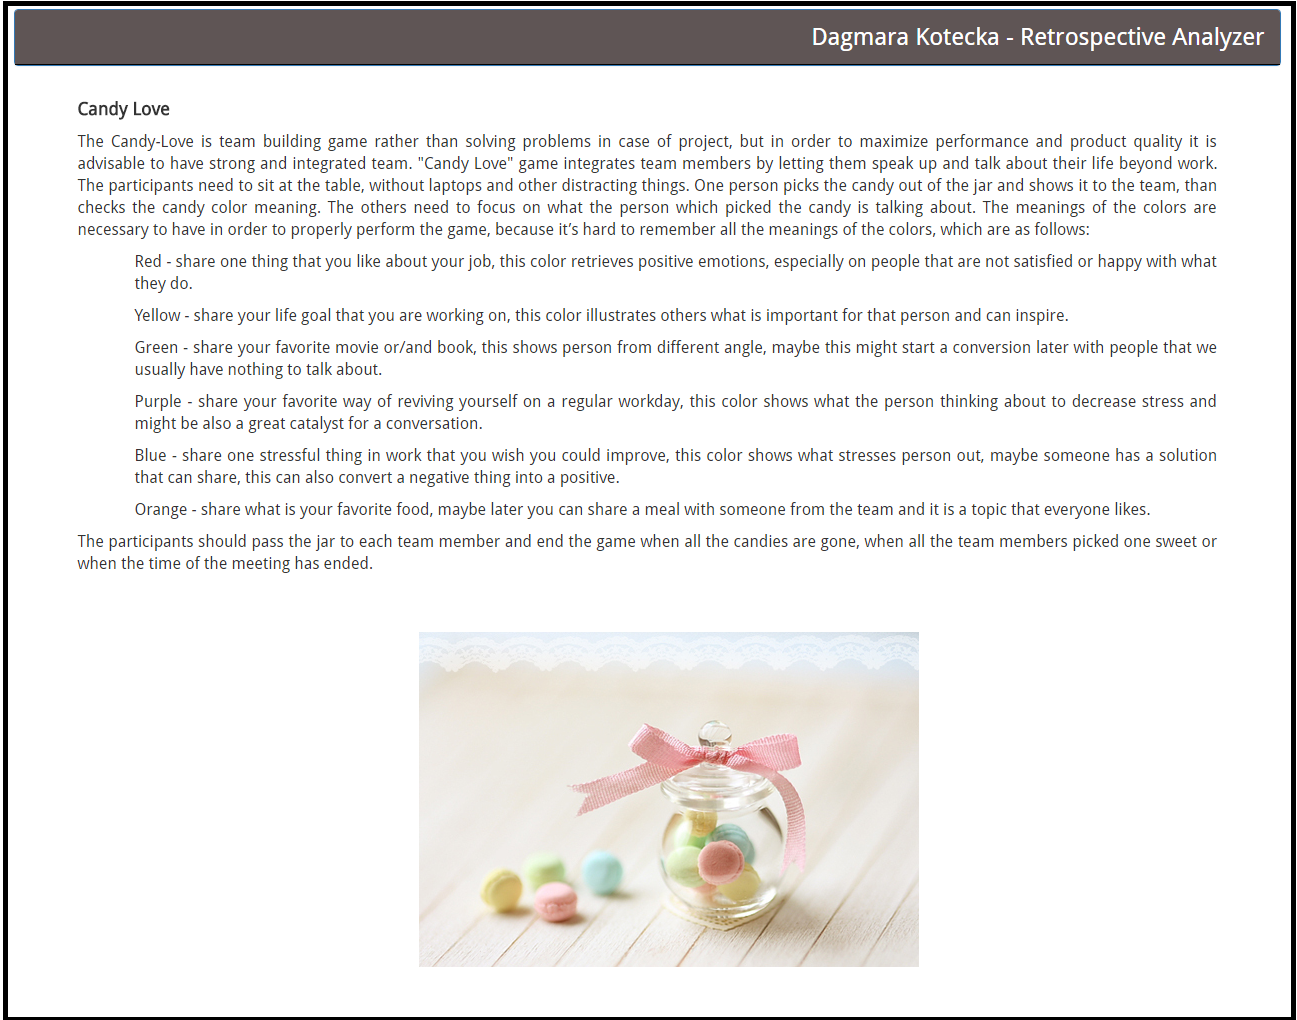
\includegraphics[width=1\textwidth]{screenshots/gameDesc.png}
\end{figure}

The use cases of the software are presented on \autoref{fig:useCases} As a developer we mean Scrum Master, Manager, Team Leaders and also Developers who lead the retrospective meetings. There are two use cases, the first one is about viewing games and the second is about answering questions.

Both the backend and frontend of the software has been written using Visual Studio 2015 with NodeJS extension on the Windows 8.1 platform. The tests has been executed on Google Chrome version 51, Internet Explorer version 11 and Mozilla Firefox version 37 browsers and the results of the evaluation were successful.

\begin{figure}[h]
\caption{System use cases}
\label{fig:useCases}
\centering
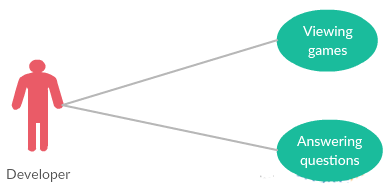
\includegraphics[width=0.5\textwidth]{img/useCases}
\end{figure}

\section{Backend architecture}

The backend is written in the NodeJS, which is an asynchronous event driven JavaScript runtime and it has been designed in order to build scalable network applications. The Google's V8 JavaScript engine interprets JavaScript in the runtime environment. NodeJS enables to create servers without using threading and it uses the model of event-driven programming that in order to signal the completion of the task uses callbacks.

The backend framework was chosen from the variety of the available possibilities for plenty of reasons. Firstly, both backend and the frontend could be written in JavaScript, that means no switching between languages and also the build process was simplified. What is more, NodeJS is distinctly faster than for example Java or PHP, there are no threads and no overheads that slow down the service.

The data is stored in Random Access Memory (RAM), because there was no need to keep it in any database. The game descriptions are being rendered by redirecting to the endpoint with the game name and the table presented on \autoref{fig:gamesPoints} with the factors is being stored in a JSON object, which is a natural part and the foundation of JavaScript and can be used without including any libraries. The other reason to not detain the data in the database is the time-consuming communication between the system and the storage. Moreover, the data that was supposed to be kept in a database was so small that creating it was pointless.

The \autoref{tab:viewingRest} presents API Rest calls made to the NodeJS server. The first call is being made in order to retrieve the game from the server, using the listed in \autoref{fig:gamesPoints} factors as parameters. The second listed in \autoref{tab:viewingRest} call is to render the page with the game description, it does not take any parameters.

\begin{table}[h]
	\caption{Rest API calls}
	\label{tab:viewingRest}
	\begin{tabularx}{\textwidth}{|X|X|X|X|X|}
	\hline
		Type of HTTP Request & URL & Parameters & On Success & Description \\ \hline
		/POST &  /{gameName} & creativity, collaboration, teammood, communication, involvement, honesty, perspective, improvement, entertainment & Returns a game & Call to server to retrieve the game after ansering on a set of questions \\ \hline
		/GET & /getGame & None & Renders Page & Rendering description page of the games. \\ \hline
	\end{tabularx}
\end{table}

For the purpose of maintaining the pages Express has been used, which is an minimal and flexible NodeJS web application framework. Thanks to Express it is easy to create a server using just a few lines. The declaration of endpoints and REST Api calls is very simple and comparing to the main competitors of Express framework, the Koa and the Hapi, it has the biggest community and is the most mature. What is more, it promotes code reuse with it's built in router.

\section{Frontend structure}

While implementing the frontend of the retrospective the main goal was to create a simple, intuitive and responsive design. In order to simplify the interface, bootstrap framework has been used. Thanks to the bootstrap framework the website scales and is properly viewed on phones, tablets and desktops with the CSS media queries. 

The choice for the framework that would ease and allow developers to create a responsive design of the responsive website has been made between two the most popular and well documented solutions. The retrieved candidates were Bootstrap and Foundation. The main aspect why the Bootstrap framework has been chosen, was the fact that we have already implemented services using it and have experience in that field. The comparison presented in the \autoref{tab:compBootFound} shows that both frameworks have very similar specifications and without the advantage of our experience in Bootstrap it would not matter which would be chosen. The main advantages of Bootstrap are the support for all the modern browsers and the bigger support community. What is more, the code is clean and readable using Bootstrap framework, moreover it is easy to find the examples and tutorials how to implement a particular element. The components on the Bootstrap site are well documented, described and explained how to use them.

\begin{table}[ht!]
\caption{Comparison between Bootstrap and Foundation}
\label{tab:compBootFound}
\begin{tabularx}{\textwidth}{|X|X|X|}
\hline
\textbf{Comparison area} & \textbf{Bootstrap} & \textbf{Foundation}  \\ \hline
Browser support & all modern web browsers & lack of Internet Explorer 8 support \\ \hline
Community support & bigger than Foundation & smaller than Bootstrap \\ \hline
Performance & similar to Foundation & similar to Bootstrap \\ \hline
Layout definition & easy & easier \\ \hline
Sizing units & pixels & rems (equals to the font size of root element)\\ \hline
Form validation & not so easy at the beginning & effortless (\textit{Abide}) \\ \hline
\end{tabularx}
\end{table}

Even though HTML has been a foundation of the web we decided to make a use of a more modern approach Jade, which has been designed in the begging for server-side templating in NodeJS, but in our solution it has been used as a short hand for HTML. Using it has made the code cleaner and there was no need to use ending tags. The Jade is using whitespaces and indentation as part of its language, so in order to properly render a page it is crucial to be careful and follow the proper syntax. What is more, Jade offers easy way to write conditions and iterators, what in result shortens the code like on example presented on \autoref{fig:jadeHtml}.

\begin{figure}[ht!]
\caption{The same layout defined in Jade and HTML}
\label{fig:jadeHtml}
\centering
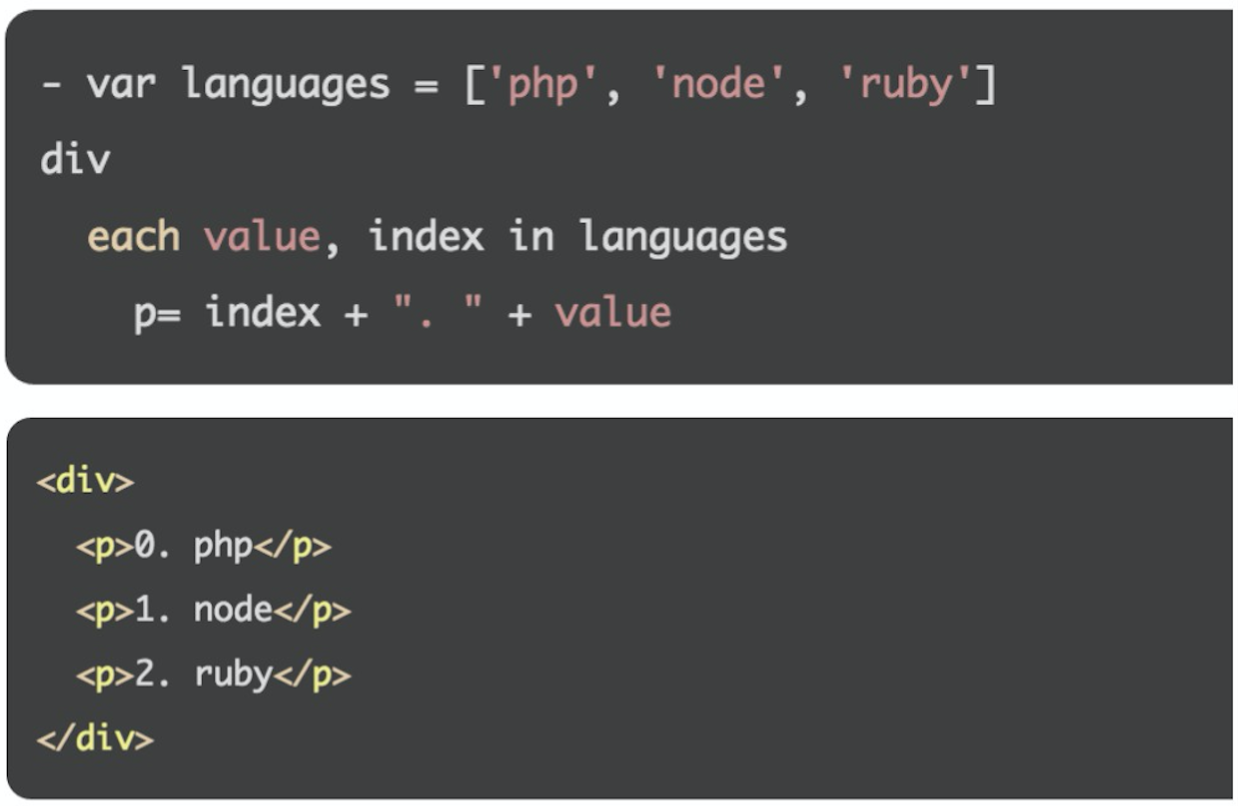
\includegraphics[width=0.5\textwidth]{img/htmlJade}
\end{figure}

\section{System evaluation}

The web service evaluation has been made in Intel Technology Poland site in Gdansk. The Scrum Master, Grzegorz Reglinski, after testing the software, has made a few suggestions. The Retrospective is the least appreciated meeting in Scrum and the task of encouraging team members to actively participate is a difficult job. Grzegorz thinks that the Retrospective Analyzer is very useful in case of supporting the leader, who performs the activity. He found the software very easy to use, the interface is intuitive, the layout is simple, does not contain any useless content. What is more, he tested the main functionality of the web-service, the game retrieval, and he was satisfied with the outcome. The answers on the input questions suited the game he wanted to get. He also noticed an easy to understand and interesting descriptions of the retrospective approaches. Grzegorz found the pictures and the description very important in order to properly perform the game. He suggested a few improvements and two out three of them have been added to the software immediately: 
\begin{enumerate}
    \item The welcome page should contain a picture of the flow, how the game retrieval functionality works. The picture express more than words. The suggested improvement is presented on \autoref{fig:welcomePageImpr}.
    \item The questions should have bigger spaces between each other and instead of a number describing the opinion a statement e.g. in place of 5 there would be "the team is very creative, has plenty of ideas and is eager to share them". The implied improvement is presented on has been added to the backlog.
    \item Each game description should contain the points evaluation presented in \autoref{fig:gamesPoints}. The suggested improvement is presented on \autoref{fig:gamePageImpr}.
\end{enumerate}

\begin{figure}[ht!]
\caption{The improved Welcome Page}
\label{fig:welcomePageImpr}
\centering
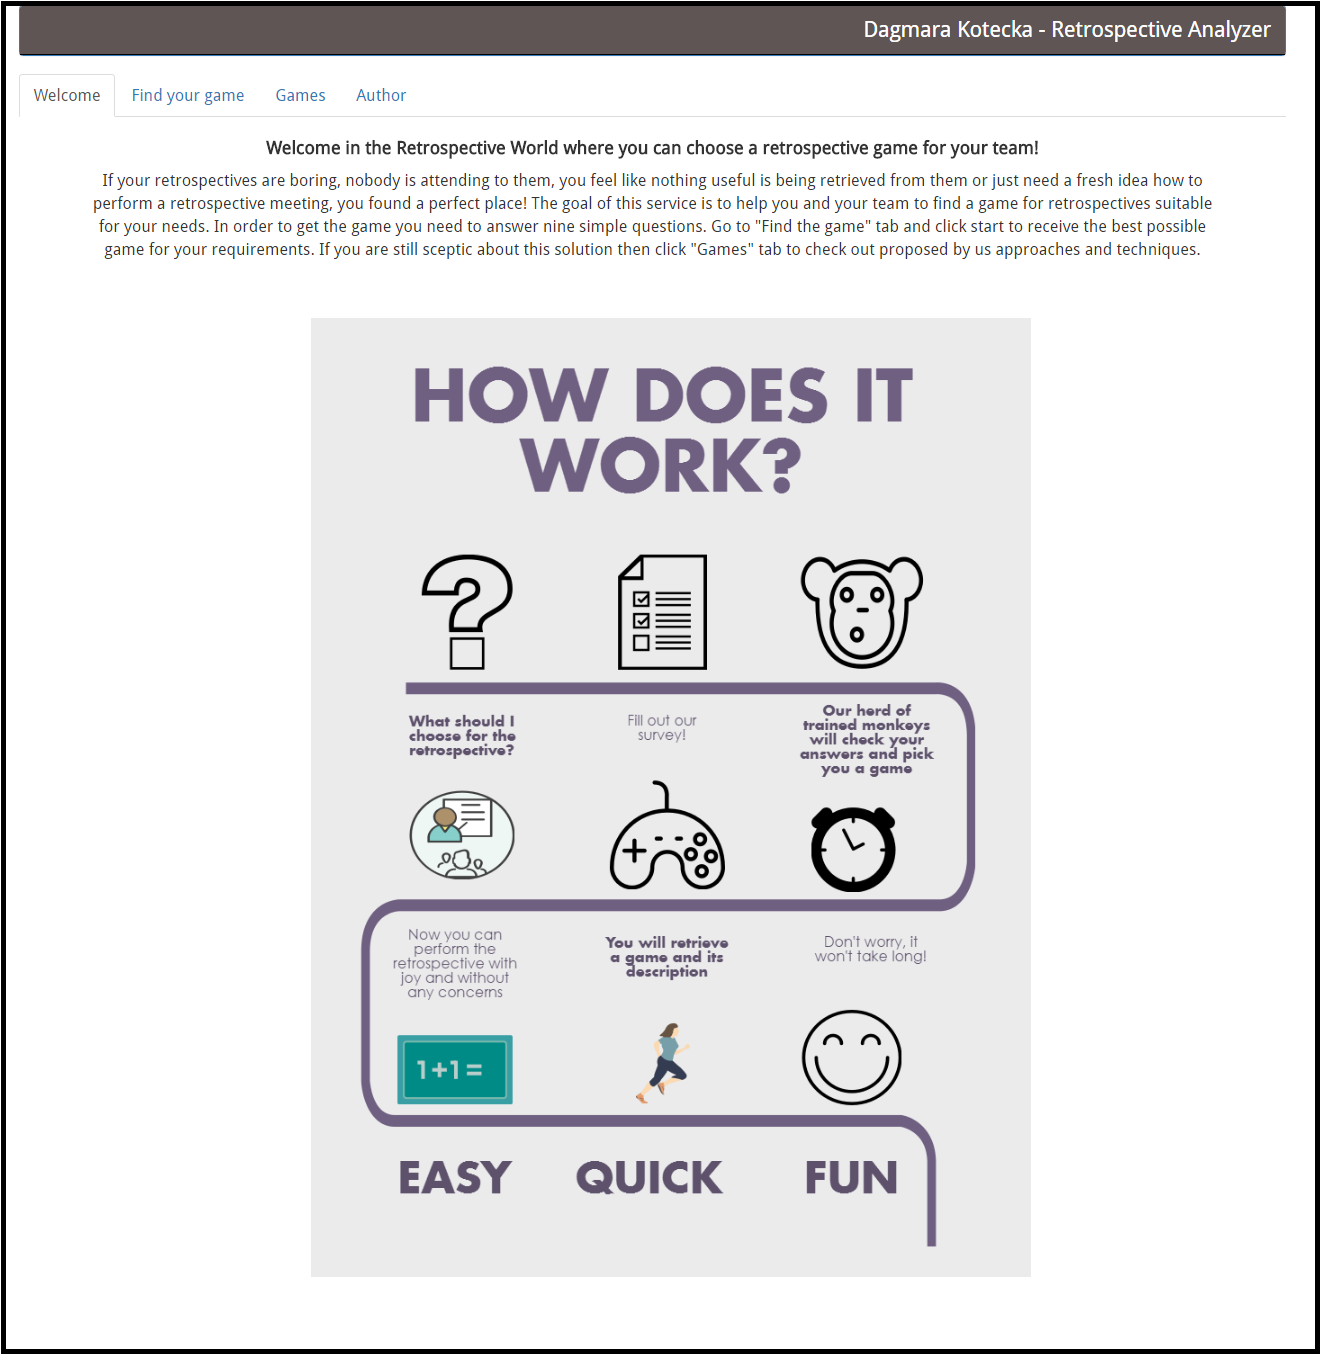
\includegraphics[width=1.0\textwidth]{img/newWelcome}
\end{figure}

\begin{figure}[ht!]
\caption{The improved Game Page with the Game Points included}
\label{fig:gamePageImpr}
\centering
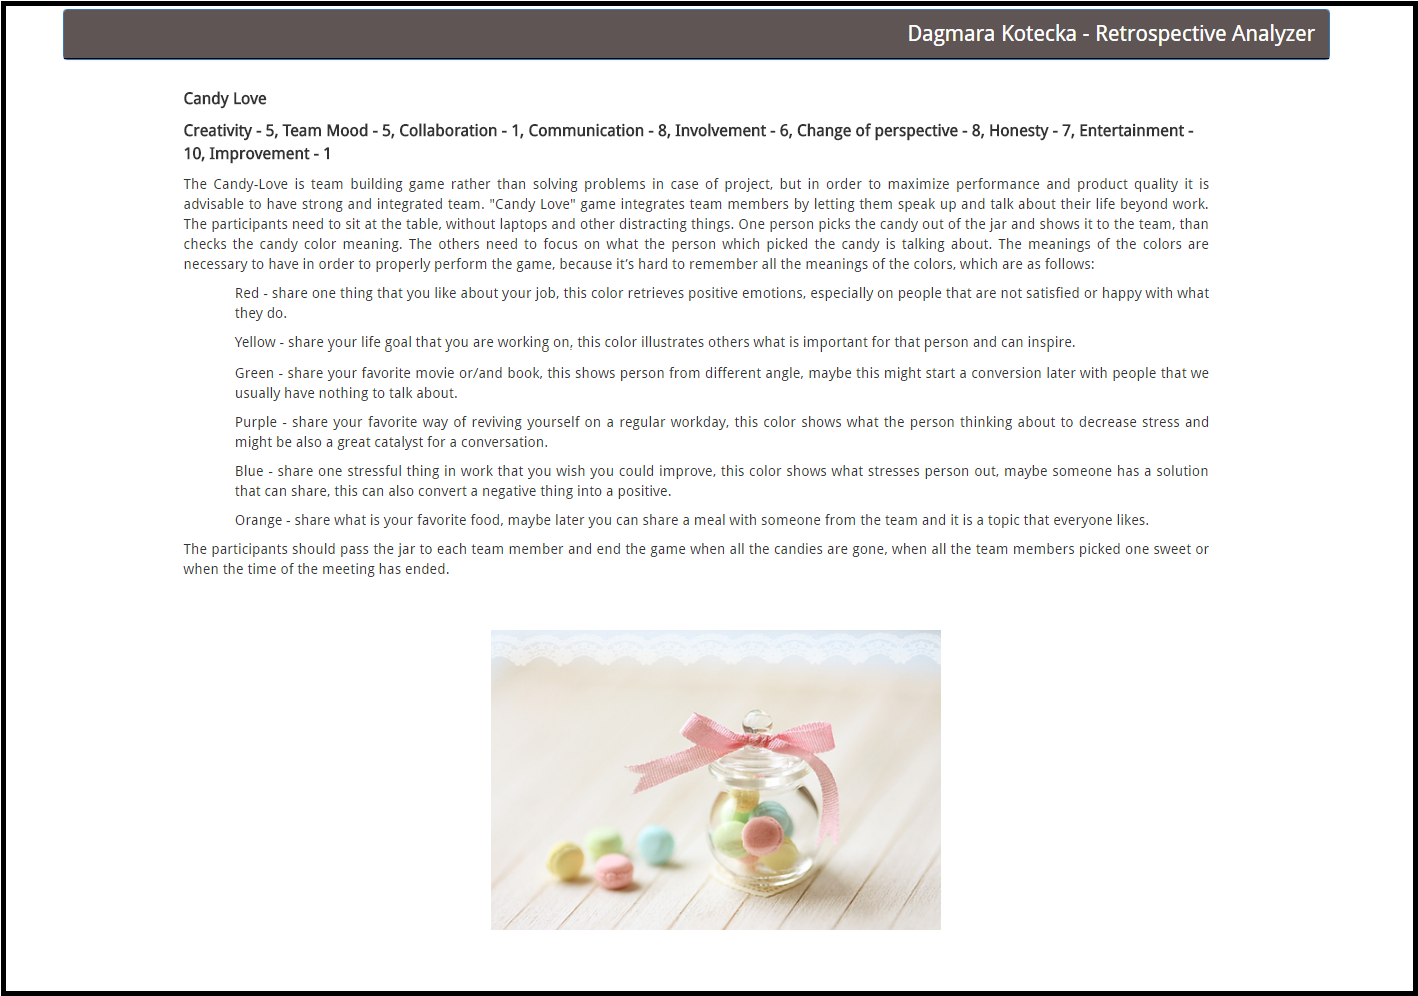
\includegraphics[width=1.0\textwidth]{img/newGame}
\end{figure}

What is more, this complementary Retrospective Analyzer web service has implemented the "must have" features in order to show how many possibilities there are to help the developers to effectively perform the Scrum Retrospective meeting. There are plenty of planned features that might make the system more functional, but as it is with the software, the system is done when the deadline comes, because the development of the service can last forever until someone says "Stop, that is enough". The possible features that might be included in the software in the future have been retrieved through valuable discussion with Grzegorz Reglinski and are as follows:
\begin{enumerate}
    \item As a scrum master, I would like the system to be extended to allow multiple user affect the result (which game will be chosen).
    \item As a scrum master, I would like to have a possibility to create separate groups for the team in order to maintain the results of each group.
    \item As a scrum master, I would like to have a admin panel where I can track the results of the game.
    \item As a user, I would like the questions to have bigger spaces between each other and instead of a number describing the opinion a statement e.g. in place of 5 there would be "the team is very creative, has plenty of ideas and is eager to share them".
\end{enumerate}



